\documentclass{article}

\usepackage{fullpage, graphicx, color, transparent, colortbl}
\usepackage[usenames, dvipsnames]{xcolor}

\begin{document}

\noindent \textbf{Keith Winstein --- Ph.D.~Thesis Proposal}

\vspace{\baselineskip}

\noindent \textbf{Thesis title: } Transport Architectures for an Evolving Internet

\vspace{\baselineskip}

In the Internet architecture, transport protocols are the glue between
an application's needs and the network's abilities. The Transmission
Control Protocol, or TCP, plays this role for the vast majority of
Internet traffic, and TCP's implementation may be the most widely used
computer program in the world. Viewed through a broader lens, the
Hypertext Transfer Protocol (HTTP) over TCP is the true
transport for most applications---including the World Wide Web,
smartphone and tablet apps, and video services like YouTube, Netflix,
and Hulu.

As the Internet has matured over the last 30 years into a global
utility, HTTP and TCP have proven extraordinarily successful. But as
the Internet's underlying networks have evolved, the transport layer
has begun showing its age. The implicit assumptions of these
protocols---and their broad applicability to most applications---have held
less and less well.

TCP was designed for a world where users have one endpoint address and
continual connectivity to a wired network with ``dumb'' gateways with
limited memory, a network whose only source of packet loss is from
gateways that run out of memory to store packets in flight and whose
only variation in performance comes from cross traffic. In TCP's
world, applications have one objective: the speedy completion of a
long-running reliable file transfer.

Not one of those design assumptions still holds. The performance of
wireless networks varies greatly in time, even in the absence of other
users.  Packet loss may occur for reasons other than gateway buffer
overflow. Users regularly ``roam'' among networks (e.g.~from one Wi-Fi
network to another, or to a cellular network), changing their IP
addresses in the process. Laptops and smaller computing devices go to
sleep or lose Internet access for hours at a time.  Gateways and
routers have considerable sophistication, large buffer memories, and
complex behavior.

Furthermore, long-running file transfers now constitute a minority of
application demands on the network. Today's network applications
represent a diverse menagerie of desires. Remote procedure calls and
user interface tools (e.g.~SSH, VNC) may send only a trickle of
traffic, but care greatly about latency. Web pages generally care
about the completion time of an ensemble of small file transfers,
often sent from independent servers. Videoconferencing programs would
like a compromise between high throughput and low delay. Batch
processing applications like MapReduce may care about the tail of the
distribution of completion time of a transaction.  Applications may
ask TCP to send information that becomes superseded or obsolete before
it is successfully acknowledged---meaning TCP should stop trying to
deliver the data reliably.

The widespread use of TCP has meant that network technologies now must
be designed to satisfy TCP's implicit assumptions about them. With my
advisor, Hari Balakrishnan, I earlier argued in a position
paper\footnote{K.~Winstein and H.~Balakrishnan, End-to-End
  Transmission Control by Modeling Uncertainty about the Network
  State, in Proceedings of ACM HotNets 2011, Cambridge, Mass.,
  November 2011} that this constraint has hampered the evolution of
the Internet, which would be freer to evolve if the transport layer's
assumptions were made explicit, and the protocol made a function of
those assumptions.

Working with collaborators at MIT, I have built three
systems that explore this type of design:

\begin{enumerate}
\item \textbf{Remy}, a tool that generates end-to-end
  congestion-control schemes automatically as a function of a
  designer's goals and assumptions about the network, allowing the
  transport layer to evolve with the network. By asking Remy to search
  for the best schemes subject to different constraints, the tool
  helps investigate the fundamental limits of decentralized control on
  a packet-switched network.

\item \textbf{Sprout}, a protocol for interactive real-time
  applications such as a videoconference, that achieves many-fold gains
  in throughput and delay compared with Skype, Facetime, Google
  Hangouts, and TCP congestion-control schemes

\item \textbf{Mosh/SSP}, a remote terminal application and protocol that
  supports roaming, intermittent connectivity, and rolling latency compensation
\end{enumerate}

Based on this experience, my thesis is that the explicit modeling of
assumptions about network behavior and user objectives by the
transport layer allows the creation of new application behaviors,
frees network technologies to evolve, and improves the experience of
real-world applications.

\subsection*{1. Remy: computer-generated congestion control}

\emph{(This section will be based on material published in
  K.~Winstein and H.~Balakrishnan, TCP ex Machina: Computer-Generated Congestion Control, in Proc.~ACM SIGCOMM 2013, Hong Kong, China, August 2013.)}

\vspace{\baselineskip}

Is it possible for a computer to discover the right rules for
congestion control in heterogeneous and dynamic networks? Should
computers, rather than humans, be tasked with developing congestion
control methods?  And just how well can we make computers perform this
task?

We investigated these questions and found that computers can design
schemes that in some cases surpass the best human-designed methods to
date, when supplied with the appropriate criteria by which to judge a
congestion-control algorithm. In my dissertation, I will discuss how
this style of transport-layer protocol design can give more freedom to
network architects and link-layer designer, and provide angles for
understanding fundamental questions about the limits of decentralized
network algorithms.

\begin{figure}
\vspace{\baselineskip}
\begin{centering}
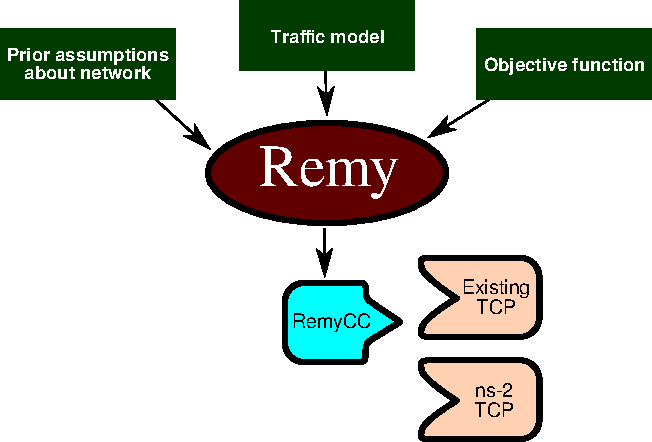
\includegraphics[width=6 cm]{remy.pdf}
\caption{Remy designs congestion-control schemes automatically to
  achieve desired outcomes. The algorithms it produces may replace
the congestion-control module of a TCP implementation, and fit into
a network library or kernel module that implements congestion
control (DCCP, SCTP, the congestion manager, application-layer
transmission control libraries, ns-2 modules, etc.).}

\end{centering}

\end{figure}

Congestion control, a fundamental problem in multi-user computer
networks, addresses the question: when should an endpoint transmit
each packet of data? An ideal scheme would transmit a packet whenever
capacity to carry the packet was available, but because there are many
concurrent senders and the network experiences variable delays, this
question isn't an easy one to answer. On the Internet, the past thirty
years have seen a number of innovative and influential answers to this
question, with solutions embedded at the endpoints (mainly in TCP)
aided occasionally by queue management and scheduling algorithms in
bottleneck routers that provide signals to the endpoints.

This area has continued to draw research and engineering effort
because new link technologies and subnetworks have proliferated and
evolved. For example, the past few years have seen an increase in
wireless networks with variable bottleneck rates; datacenter networks
with high rates, short delays, and correlations in offered load; paths
with excessive buffering (now called ``bufferbloat''); cellular
wireless networks with highly variable, self-inflicted packet delays;
links with non-congestive stochastic loss; and networks with large
bandwidth-delay products. In these conditions, the classical
congestion-control methods embedded in TCP can perform poorly, as many
papers have shown.

Without the ability to adapt its congestion-control algorithms to new
scenarios, TCP's inflexibility constrains architectural evolution, as
we noted in the 2011 position paper.\footnote{Above, footnote 1.}
Subnetworks and link layers are typically evaluated based on how well
TCP performs over them.  This scorecard can lead to perverse behavior,
because TCP's network model is limited. For example, because TCP
assumes that packet losses are due to congestion and reduces its
transmission rate in response, some subnetwork designers have worked
hard to hide losses. This often simply adds intolerably long packet
delays. One may argue that such designs are misguided, but the
difficulties presented by ``too-reliable'' link layers have been a
perennial challenge for 25 years and show no signs of abating. With
the rise of widespread cellular connectivity, these behaviors are
increasingly common and deeply embedded in deployed infrastructure.

The designers of a new subnetwork may well ask what they should do to
make TCP perform well. This question is surprisingly hard to answer,
because the so-called teleology of TCP is unknown: exactly what
objective does TCP congestion control optimize? TCP's dynamic
behavior, when competing flows enter and leave the network, remains
challenging to explain.  In practice, the need to ``make
TCP perform well'' is given as a number of loose guidelines, such as
IETF RFC 3819, which contains dozens of pages of
qualitative best current practice. The challenging and subtle nature
of this area means that the potential of new subnetworks and network
architectures is often not realized.

\subsection*{Design overview}

How should we design network protocols that free subnetworks and links
to evolve freely, ensuring that the endpoints will adapt properly
\emph{no matter what} the lower layers do?  We believe that the best
way to approach this question is to take the design of specific
algorithmic mechanisms out of the hands of human designers (no matter
how sophisticated!), and make the end-to-end algorithm be a function
of the desired overall behavior.

%These actions should not
%depend on explicit signals about unusual network behaviors, e.g., if a
%new network were to reorder packets because of multi-path routing,
%endpoints should not have to be notified.

As with Mosh and Sprout, we start by explicitly stating an 
  objective for congestion control; for example, given an unknown
number of users, we may optimize some function of the per-user
throughput and packet delay, or a summary statistic such as average
flow completion time. Then, instead of writing down rules by hand for
the endpoints to follow, we start from the desired objective and work
backwards in three steps:

%\item We specify a utility function that quantifies the
%  benefit to each user of the network. As in other work, this is
%  generally a concave function of average throughput, so that a fair
%  allocation is preferred. We then subtract a concave function of the
%  user's average delay, to penalize induced latency.

%We have developed an alternate approach for end-to-end resource
%management and transmission control. 

\begin{enumerate}

\item First, model the protocol's prior assumptions about the network;
  i.e., the ``design range'' of operation. This model
  may be different, and have different amounts of uncertainty, for a
  protocol that will be used exclusively within a data center,
  compared with one intended to be used over a wireless link or one
  for the broader Internet. A typical model specifies upper and lower
  limits on the bottleneck link speeds, non-queueing delays, queue
  sizes, and degrees of multiplexing.
%The model represents the
%  designer's prior knowledge about the networks that the protocol will
%  encounter.

\item Second, define a traffic model for the offered load given to
  endpoints. This may characterize typical Web traffic, video
  conferencing, batch processing, or some mixture of these. It may
  be synthetic or based on empirical measurements.

\item Third, use the modeled network scenarios and traffic to design a
  congestion-control algorithm that can later be executed on endpoints.

\end{enumerate}

We have developed an optimization tool called Remy that takes these
models as input, and designs a congestion-control algorithm that tries
to maximize the total expected value of the objective function, measured over the set of
network and traffic models. The resulting pre-calculated, optimized
algorithm is then run on actual endpoints; no further learning happens
after the offline optimization. The optimized algorithm is run as part
of an existing TCP sender implementation, or within any
congestion-control module. No receiver changes are necessary (as of
now).

\subsection*{Summary of results}

We have implemented Remy. Running on a 48-core server at MIT, Remy
generally takes a few hours of wall-clock time (one or two CPU-weeks)
to generate congestion-control algorithms offline that work on a wide
range of network conditions.

Our main results from several simulation experiments
with Remy are as follows:

\begin{enumerate}

\item For networks broadly consistent with the assumptions provided to
  Remy at design time, the machine-generated algorithms dramatically
  outperform existing methods, including TCP Cubic, Compound TCP, and
  TCP Vegas.

\item Comparing Remy's algorithms with schemes that require
  modifications to network gateways, including Cubic-over-sfqCoDel and
  XCP, Remy generally matched or surpassed these schemes, despite
  being entirely end-to-end.

\item We measured the tradeoffs that come from specificity in the
  assumptions supplied to Remy at design time. As expected,
  more-specific prior information turned out to be helpful when it was
  correct, but harmful when wrong. We found that RemyCC schemes
  performed well even when designed for an order-of-magnitude
  variation in the values of the underlying network parameters.
\end{enumerate}

\begin{figure}
\begin{centering}
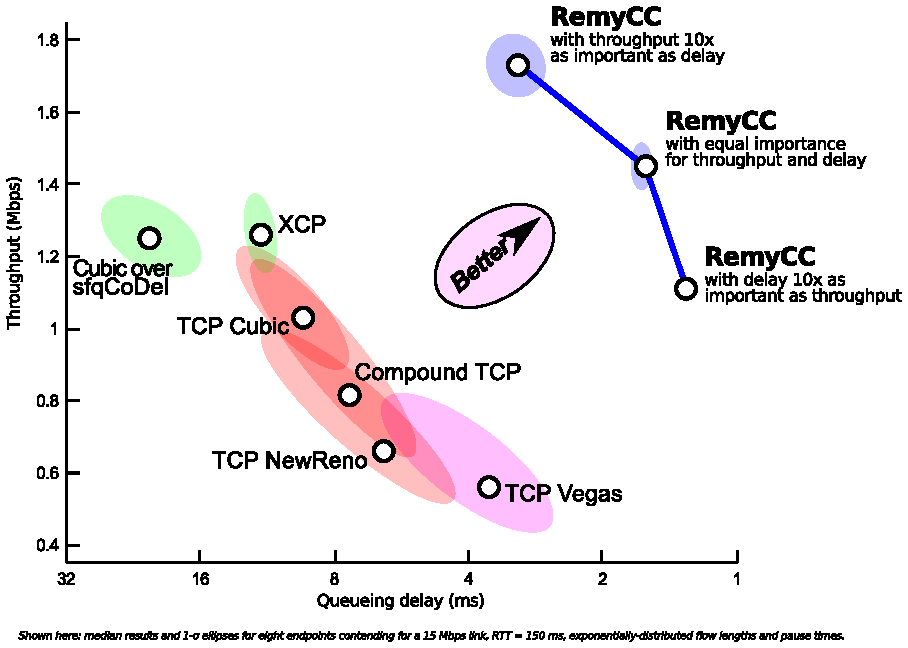
\includegraphics[width=8 cm]{remy-hero-chart-convert2.pdf}
\caption{Results for each of the schemes over a 15~Mbps dumbbell
topology with n=8 senders, each alternating between flows
of exponentially-distributed byte length (mean 100 kilobytes)
and exponentially-distributed off time (mean 0.5~s). Medians
and 1-$\sigma$ ellipses are shown. The blue line represents the efficient
frontier, which here is defined entirely by the RemyCCs.}
\label{f:remy-fig4}
\end{centering}
\end{figure}

On a simulated 15~Mbps fixed-rate link with eight senders contending
and an RTT of 150~ms, a computer-generated congestion-control
algorithm achieved the following improvements in median throughput and
reductions in median queueing delay over these existing protocols. The
results are plotted in Figure~\ref{f:remy-fig4}.

\vspace{\baselineskip}

\begin{centering}
{\footnotesize
\begin{tabular}{|l|c|c|}
\hline
Protocol & Median speedup & Median delay reduction \\
\hline
\hline
Compound & $2.1\times$ & $2.7\times$ \\
NewReno & $2.6\times$ & $2.2\times$ \\
Cubic & $1.7\times$ & $3.4\times$ \\
Vegas & $3.1\times$ & $1.2\times$ \\
\hline
Cubic/sfqCoDel & $1.4\times$ & $7.8\times$ \\
XCP & $1.4\times$ & $4.3\times$ \\
\hline
\end{tabular}
}

\end{centering}

\vspace{\baselineskip}

In a trace-driven simulation of the Verizon LTE downlink with four
senders contending, the \emph{same} computer-generated protocol achieved these
speedups and reductions in median queueing delay:

\vspace{\baselineskip}

\begin{centering}
{\footnotesize
\begin{tabular}{|l|c|c|}
\hline
Protocol & Median speedup & Median delay reduction \\
\hline
\hline
Compound & $1.3\times$ & $1.3\times$ \\
NewReno & $1.5\times$ & $1.2\times$ \\
Cubic & $1.2\times$ & $1.7\times$ \\
Vegas & $2.2\times$ & $0.44\times \downarrow$ \\
\hline
Cubic/sfqCoDel & $1.3\times$ & $1.3\times$ \\
XCP & $1.7\times$ & $0.78\times \downarrow$ \\
\hline
\end{tabular}
}

\end{centering}

\subsection*{Remy as a tool for network science}

In addition to its utility as a tool for constructing
congestion-control algorithms, Remy is an aid for understanding
the limits and structure of distributed networking problems. In my
dissertation, I will report the results of our ongoing computational
experiments that use Remy to address several open questions in network
science and the optimization of decentralized algorithms:

\begin{figure}
\begin{centering}
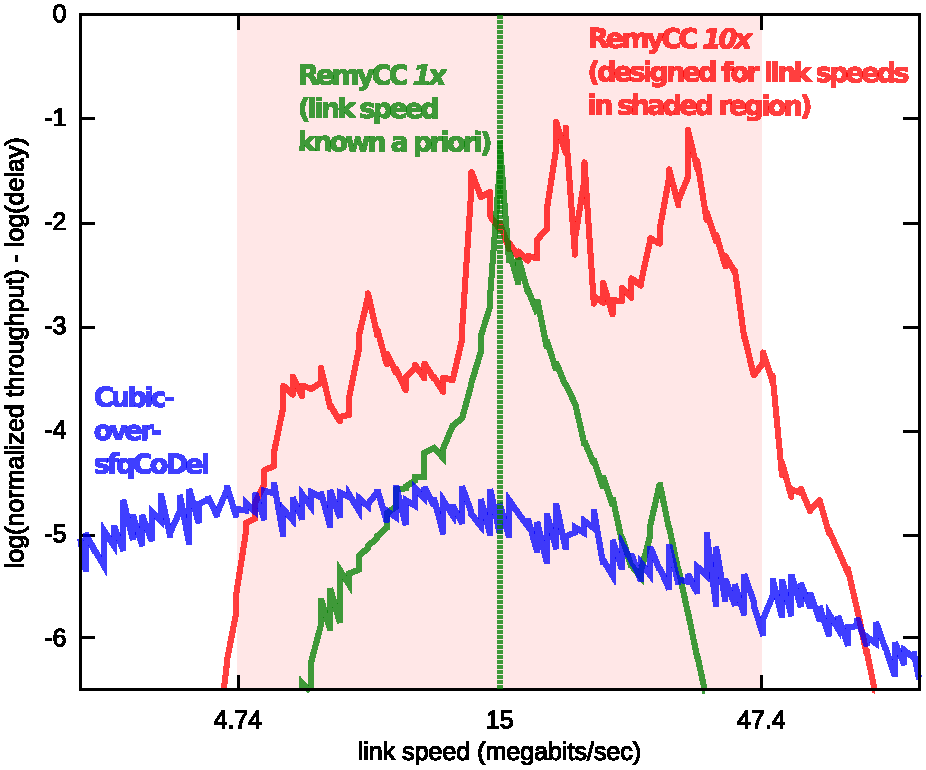
\includegraphics[width=8 cm]{spec-web.pdf}
\caption{How helpful is prior information about the network? Here we
  show the performance of two end-to-end RemyCCs that were designed
  with different prior information about the network, compared with an
  in-network algorithm (Cubic-over-sfqCoDel), as the link speed
  varies. Despite running only at the sender, the RemyCCs each
  outperform Cubic-over-sfqCoDel over almost their entire design
  ranges. But when a RemyCC's assumptions aren't met, performance
  deteriorates. The extent to which there is a tradeoff between
  the ``operating range'' and performance of a RemyCC is so far unresolved.}
\label{f:remy-spec}
\end{centering}
\end{figure}

\begin{itemize}

\item How helpful is prior information about a network? To what extent
  are the RemyCCs' gains (relative to human-designed algorithms) due
  to the benefits of explicit optimization towards an objective,
  vs.~simply to the narrowed ``operating range'' implied by the stated
  assumptions?  Is there a tradeoff between operating range and
  performance---in other words, if we design a RemyCC for a broader
  and broader range of network conditions, does its performance
  necessarily get worse and worse (Figure~\ref{f:remy-spec})? Along
  the same lines: \emph{can} we successfully design a RemyCC that
  still beats TCP over a 10,000-fold range of throughputs or
  round-trip times?

\item To what extent is the end-to-end congestion-control problem
  decomposable? If we wish to design a RemyCC that works well on a
  complex network (e.g.~the actual Internet), must we also optimize on
  a model of that complex network? What is the penalty associated with
  optimizing for a simple model, but then running a
  computer-engineered solution in the real world? How can we explain
  or put bounds on this cost, of using a simple model in a complex world?

\item Which congestion signals (in machine-learning terms, which
  features) are helpful in different network scenarios (e.g.~high
  multiplexing, high BDP) and which aren't? Can we develop a general theory
  to predict which features will be helpful, when?

\item What is the ``cost of compatibility''? How much does it hurt the performance
of a RemyCC if we demand that it also achieve the right result when competing
against ``buffer-filling'' TCP algorithms?

\item How can we quantify the ``cost of coexistence''? How well can we co-optimize
  a pair of RemyCCs that satisfy different objectives, so as to
  achieve an appropriate division of network resources---even when
  each RemyCC is uncertain about how many other RemyCCs are contending
  for the same bottleneck, or what objective they are each trying to
  optimize.

\end{itemize}

\subsection*{2. Sprout: using forecasts of network variation to achieve an explicit objective}

\emph{(This section will be based on material published in
  K.~Winstein, A.~Sivaraman, and H.~Balakrishnan, Stochastic Forecasts
  Achieve High Throughput and Low Delay over Cellular Networks, in
  Proc.~USENIX NSDI 2013, Lombard, Ill., April 2013.)}

\vspace{\baselineskip}

Cellular wireless networks have become a dominant mode of Internet
access. These mobile networks, which include LTE and 3G (UMTS and
1xEV-DO) services, present new challenges for network applications,
because they behave differently from wireless LANs and from the
Internet's traditional wired infrastructure.

Cellular wireless networks experience rapidly varying link rates
and occasional multi-second outages in one or both directions,
especially when the user is mobile. As a result, the time it takes to
deliver a network-layer packet may vary significantly, and may include
the effects of link-layer retransmissions. Moreover, these networks
schedule transmissions after taking channel quality into account, and
prefer to have packets waiting to be sent whenever a link is
scheduled. They often achieve that goal by maintaining deep packet
queues. The effect at the transport layer is that a stream of packets
experiences widely varying packet delivery rates, as well as variable,
sometimes multi-second, packet delays.

For an interactive application such as a videoconferencing program
that requires both high throughput and low delay, these conditions are
challenging. If the application sends at too low a rate, it will waste
the opportunity for higher-quality service when the link is
doing well. But when the application sends too aggressively, it
accumulates a queue of packets inside the network waiting to be
transmitted across the cellular link, delaying subsequent
packets. Such a queue can take several seconds to drain, destroying
interactivity (Figure~\ref{fig:skypevssprout}).

Experiments with Microsoft's Skype, Google's Hangout, and Apple's
Facetime running over traces from commercial 3G and LTE networks show
the shortcomings of the transport protocols in use and the lack of
adaptation required for a good user experience.
%(\S\ref{s:problem}). 
The transport protocols deal with rate variations in a reactive
manner: they attempt to send at a particular rate, and if all goes
well, they increase the rate and try again. They are slow to
decrease their transmission rate when the link has deteriorated, and as a
result they often create a large backlog of queued packets in the
network. When that happens, only after several seconds and a
user-visible outage do they switch to a lower rate.

\begin{figure}
\begin{centering}
\footnotesize\def\svgwidth{8 cm}\input{newfigure1.pdf_tex}
\caption{Skype and Sprout on the Verizon LTE downlink trace. For Skype, overshoots in throughput lead to large standing queues. Sprout has an explicit objective: send as much as possible, but keep each
packet's delay less than 100~ms with 95\% probability.}
\label{fig:skypevssprout}
\end{centering}
\end{figure}

By contrast, {\em Sprout} is a transport protocol designed to satisfy
a particular objective on behalf of interactive applications on
variable-quality networks. Sprout uses the receiver's observed packet
arrival times as the primary signal to determine how the network path
is doing, rather than the packet loss, round-trip time, or one-way
delay. Moreover, instead of the traditional reactive approach where
the sender's window or rate increases or decreases in response to a
congestion signal, the Sprout receiver makes a short-term forecast (at
times in the near future) of the bottleneck link rate using
probabilistic inference.  From this model, the receiver predicts how
many bytes are likely to cross the link within several intervals in
the near future with at least 95\% probability. The sender uses this
forecast to transmit its data, bounding the risk that the queuing
delay will exceed some threshold, and maximizing the achieved
throughput within that constraint.

We conducted a trace-driven experimental evaluation using data
collected from four different commercial cellular networks (Verizon's
LTE and 3G 1xEV-DO, AT\&T's LTE, and T-Mobile's 3G UMTS). We compared
Sprout with Skype, Hangout, Facetime, and several TCP
congestion-control algorithms, running in both directions (uplink and
downlink).

The following table summarizes the average relative throughput
improvement and reduction in self-inflicted queueing delay for Sprout
compared with the various other schemes, averaged over all four
cellular networks in both directions. Metrics where Sprout did not
outperform the existing algorithm are highlighted in red:

\vspace{\baselineskip}

\begin{centering}

\noindent \begin{tabular}{|l|c|c|}
\hline
App/protocol & Avg.~speedup & Delay reduction \\
& \footnotesize{vs.~Sprout} & \footnotesize{(from avg.~delay)}\\
\hline
\hline
\cellcolor{blue!20}Sprout & \cellcolor{blue!20}$1.0\times$ & \cellcolor{blue!20}$1.0\times$ (0.32~s) \\
\hline
Skype & $2.2\times$ & $7.9\times$ (2.52~s) \\
Hangout & $4.4\times$ & $7.2\times$ (2.28~s) \\
Facetime & $1.9\times$ & $8.7\times$ (2.75~s) \\
\hline
Compound & $1.3\times$ & $4.8\times$ (1.53~s) \\
TCP Vegas & $1.1\times$ & $2.1\times$ (0.67~s) \\
LEDBAT & $1.0\times$ & $2.8\times$ (0.89~s) \\
Cubic & \cellcolor{red!20}$0.91\times$ & $79\times$ (25~s)\\
\hline
Cubic-CoDel\footnote{Cubic-CoDel indicates TCP Cubic running over the CoDel
queue-management algorithm, which would be implemented in the
carrier's cellular equipment to be deployed on a downlink, and in
the baseband modem or radio-interface driver of a cellular phone for an
uplink.} & \cellcolor{red!20}$0.70\times$ & $1.6\times$ (0.50~s) \\
%CUBIC/CoDel & & \\
%Compound/CoDel & & \\
\hline
\end{tabular}

\end{centering}

\vspace{\baselineskip}

The Sprout experience suggests that modeling a network's state
explicitly, albeit with a simplified, imperfect model, and with the
aim of achieving a particular objective, can produce many-fold
improvements on conventional metrics over contemporary systems.

\subsection*{3. Mosh (mobile shell) and the State Synchronization Protocol}

\emph{(This section will be based on material published in K.~Winstein
  and H.~Balakrishnan, Mosh: An Interactive Remote Shell for Mobile
  Clients, in Proc.~USENIX Annual Technical Conference 2012, Boston,
  Mass., June 2012.)}

\vspace{\baselineskip}

Remote terminal applications are almost as old as packet-switched data
networks. Starting with RFC 15 in 1969, protocols like TELNET, SUPDUP,
and BSD's rlogin and rsh have played an important role in the
Internet's development. The most popular such application today is the
Secure Shell, or SSH.

SSH has two weaknesses that can make it unpleasant. First, because SSH
and previous remote terminals run over TCP, they don't support roaming
between IP addresses, or generally preserve sessions when connectivity is
intermittent.
%connectivity while data is pending. 
A laptop will happily suspend for a commute to work, but after wakeup
its SSH sessions will have frozen or died.

Second, SSH operates strictly in character-at-a-time mode, with all
echoes and line editing performed by the remote host.  As a result,
its interactive performance can be poor over wide-area wireless (e.g.,
EV-DO, UMTS, LTE) or transcontinental networks (e.g., to cloud
computing facilities or remote data centers), and sessions are almost
unusable over
%marginal
paths with non-trivial packet loss.  
%On transcontinental paths (e.g.,
%to cloud computing facilities or remote data centers) or across
%commercial wide-area wireless networks (e.g., EV-DO, UMTS, LTE),
%round-trip latency can exceed hundreds of milliseconds when
%unloaded. 

When loaded or when the signal-to-noise ratio is low, delays on many
wireless networks reach several \textit{seconds} because of deep
packet queues (``bufferbloat'') or over-zealous link-layer
retransmissions. Many home networks also suffer from
multi-second delays under load. Trying to type, or correct a typo,
over such networks is unpleasant.

Mosh (mobile shell) is addressed at both problems. Mosh is a
remote terminal application that supports IP roaming, intermittent
connectivity, and marginal network connections. Mosh performs
predictive client-side echoing and line editing without any change to
server software, and without regard to which application is running.
Mosh makes remote servers feel more like the local computer, because
most keystrokes are reflected immediately on the user's display---even
in full-screen programs like a text editor or mail reader.

These features are possible because Mosh operates at a different layer
from SSH\@. While SSH conveys an octet-stream to TCP, and eventually
to a separate client-side terminal emulator to be interpreted and
rendered in cells on the screen, Mosh contains a server-side terminal
emulator and uses a new transport protocol---the State Synchronization
Protocol---to synchronize terminal screen states over the network,
using the principle of application-layer framing.

Because both the server and client maintain an image of the screen
state, Mosh can support intermittent connectivity and local editing,
and can adjust its network traffic (even superseding screen states
that are no longer important) to avoid filling network buffers on slow
links. As a result, unlike in SSH, in Mosh ``Control-C'' always works
to cease output from a runaway process within an RTT.

Giving SSP the flexibility to send the packet that best advances the
user's objective---in this case, low UI latency---leads to better
application behavior:

\begin{itemize}

\item SSP implements ``single-packet roaming,'' which allows the client to
switch public IP addresses and keep its connection by sending one
packet from the new address---without needing to know that it has
switched IP addresses at all.

\item The protocol also uses a novel technique, called ``pretransmissions,''
to code opportunistically against packet loss. When formulating a
transmission to the receiver, the sender will normally use the most
recent state transmitted as a predicate (even if this state has not
yet been acknowledged, as long as it has not timed out). This is what
TCP does, by sending only new data in each segment, and this policy
represents a gamble---if the older segment does not arrive, neither
transmission will be useful to the receiver without a retransmission.

Instead, SSP may optionally choose to base its transmission only on
a state that has actually been acknowledged by the receiver. This will
typically require more bits on the wire, but usually by only a modest
amount compared with framing overhead. The benefit is that the new
transmission is sufficient to update the receiver to the current state
by itself, even if previous in-flight transmissions are lost.

\item In addition, Mosh introduces the technique of ``rolling latency
  compensation'' to improve the user's experience when interacting
  with a server-side application across the network. The Mosh client
  runs a predictive model of the application in the background, and
  uses the model to do intelligent client-side echoing and line
  editing. When confident in a prediction, Mosh will display it to the
  user, but underlined. As predictions are confirmed, Mosh removes the
  underline. The effect is a sliding ``prediction window'' of
  keystrokes shown locally but not yet confirmed by the server.

  According to data we have collected from contributing users, more
  than two-thirds of the keystrokes in a typical Unix session can be
  displayed instantly with a conservative model of application
  behavior (Figure~\ref{f:moshcdfs}). Mosh's empirical approach to
  local echo works in full-screen programs like a text editor or mail
  reader as well as at the command line.

\end{itemize}

\begin{figure}
\begin{centering}
\def\svgwidth{8 cm}\footnotesize\input{cdfs.pdf_tex}
\caption{In 40 hours of user-submitted sessions, Mosh successfully
  predicted and displayed 70\% of user keystrokes immediately. The error rate was less than 1\%.}
\label{f:moshcdfs}
\end{centering}
\end{figure}

We have implemented Mosh in C++ and published it as free software. It
is in wide deployment and has been packaged for or included in Debian
GNU/Linux, Ubuntu, Fedora, Red Hat EPEL, Gentoo, Arch Linux, FreeBSD,
NetBSD, OpenBSD, Android, Cygwin, Homebrew, MacPorts, and OpenSolaris.

\section*{4. Conclusion and Timeline}

My thesis is that the explicit modeling of assumptions about network
behavior and user objectives by the transport layer allows the
creation of new application behaviors, frees network technologies to
evolve, and improves the experience of real-world applications.

I propose to defend and deliver the dissertation in time for
graduation in June 2014. The Mosh and Sprout sections will largely
be based on the published conference papers about those systems. The Remy
section will also be based on its conference paper (SIGCOMM 2013),
with the addition of our further work on Remy that, along with my
co-authors, we are submitting this coming January for review at
SIGCOMM 2014.

In addition to the above, I am working on a project to produce an
Internet stored-video system (similar to YouTube, Netflix, and Amazon
Streaming) from first principles, based again on the principle of
explicit objectives and network modeling, as well as a new design for
``networked video coding.'' If this work is successful, I would plan to
include it as a chapter in the dissertation.

\end{document}
